%%==================================================================%%
%% Author : Tejedo Gonz�lez, Daniel                                 %%
%%          S�nchez Barreiro, Pablo                                 %%
%% Version: 1.0, 25/11/2012                                         %%                   %%                                                                  %%
%% Memoria del Proyecto Fin de Carrera                              %%
%% Sintaxis abstracta, archivo ra�z                                       %%
%%==================================================================%%

\chapterheader{Creaci�n de la sintaxis abstracta}{Creaci�n de la sintaxis abstracta}
\label{chap:metamodelo}

A partir de aqu�, los siguientes cap�tulos tratan de describir en detalle cada una de las tareas expuestas en la planificaci�n del proyecto. Evidentemente, se ha obviado la tarea de documentaci�n, pues no requiere explicaci�n alguna. Este cap�tulo en concreto versa sobre la creaci�n de la sintaxis abstracta del lenguaje, as� como cada una de las subtareas subyacentes.

\chaptertoc

\section{Captura de requisitos}
\label{sec:meta:requisitos}
%%==================================================================%%
%% Author : Tejedo Gonz�lez, Daniel                                 %%
%%          S�nchez Barreiro, Pablo                                 %%
%% Version: 1.0, 25/11/2012                                         %%
%% Version: 2.0, 06/02/2013                                         %%
%%                                                                  %%
%% Memoria del Proyecto Fin de Carrera                              %%
%% Sintaxis abstracta, requisitos                                   %%
%%==================================================================%%

El primer paso para desarrollar nuestro lenguaje era conocer qu� aspecto deb�a tener nuestro lenguaje y qu� restricciones deb�a satisfacer. Es decir, en primer lugar debemos realizar un proceso que podemos denominar de captura de requisitos para poder comprender qu� es lo que tiene que hacer exactamente el lenguaje que se pretende crear.

Concretamente nuestro lenguaje hab�a sido pr�cticamente definido por el profesor Pablo S�nchez, del Departamento de Matem�ticas, Estad�stica y Computaci�n de la Universidad de Cantabria, mediante notaci�n BNF. Dicha gram�tica, se muestra en la Figura~\ref{fig:constraintBNF}. Las ideas subyacentes a dicho lenguaje son las que se describen a continuaci�n. 

\begin{figure}[!tb]
    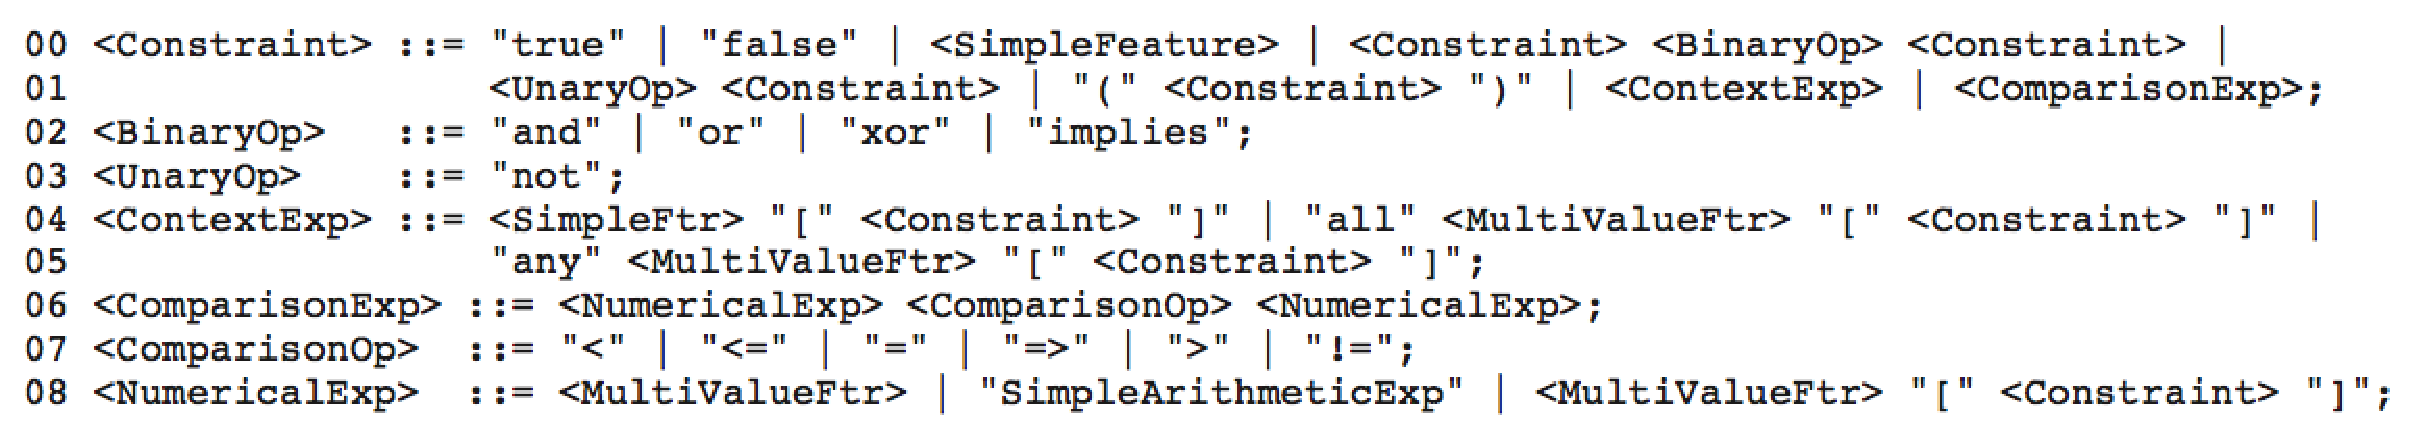
\includegraphics[scale=0.3]{metamodelo/constraintBNF.eps}
    \caption{Gram�tica en notaci�n BNF del lenguaje HCL}
    \label{fig:constraintBNF}
\end{figure}

En dicho lenguaje, una \emph{restricci�n} es una expresi�n l�gica que se puede evaluar a verdadero o falso. Una restricci�n puede ser simplemente un literal, es decir, $true$ o $false$, que se evaluar� a verdadero y falso respectivamente. Una restricci�n tambi�n puede ser una caracter�stica simple, es decir, una caracter�stica que puede aparecer en las configuraciones como m�ximo una vez. Una caracter�stica simple se eval�a a verdadero si ha sido seleccionada, y a falso en caso contrario.

Las caracter�sticas clonables son aquellas que pueden ser seleccionadas m�s de una vez en las configuraciones que construyamos sobre nuestro �rbol de caracter�sticas. Una caracter�stica clonable se eval�an como un n�mero entero positivo, incluido el cero. Ese n�mero representa el n�mero de clones que la caracter�stica posee dentro de una configuraci�n, o dicho de otro modo, el n�mero de veces que ha sido seleccionada. El hecho de que se eval�en como si fueran n�meros permite la inclusi�n de operaciones de comparaci�n entre distintas caracter�sticas clonables. Las operaciones de comparaci�n que se han de implementar son las siguientes: $<$,$<$=,$>$,$>=$,$=$,$!=$. Adem�s, tambi�n se puede utilizar el valor de las caracter�sticas clonables para implementar operaciones aritm�ticas b�sicas, tales como la suma, la resta, la multiplicaci�n y la divisi�n. Estas expresiones a su vez se pueden utilizar como subexpresiones, u operandos, dentro de las operaciones de comparaci�n. Las expresiones de comparaci�n se eval�an a verdadero o falso, y tambi�n pueden ser usadas como subexpresiones para crear expresiones l�gicas m�s complejas.

%%============================================================================%%
%% NOTA(Pablo) : Poner un ejemplo de este tipo de restricciones y explicarlas %%
%%============================================================================%%

Tal y como muestra la Figura~\ref{fig:constraintBNF}, una restricci�n tambi�n puede especificar un contexto concreto en el que poder evaluarla. Esto puede hacerse de varias maneras. Se puede especificar un contexto para una restricci�n poni�ndola entre corchetes y especificando el nombre de una caracter�stica al principio de la expresi�n. La caracter�stica usada como contexto puede ser tanto simple como m�ltiple. En el primer caso, la restricci�n s�lo ser� evaluada en el sub�rbol de la configuraci�n cuya ra�z sea la caracter�stica especificada.

%%============================================================================%%
%% NOTA(Pablo) : Poner un ejemplo y explicarlo                                %%
%%============================================================================%%

En el segundo caso entran en juego los operadores $all$ (para todo) y $any$ (existe). La operaci�n $all$ solo se evaluar� a verdadero si la restricci�n entre corchetes se cumple para todas las instancias de la caracter�stica clonable que act�a como contexto. En caso contrario, la operaci�n se evaluar� a falso. La operaci�n $any$ se evaluar� a verdadero si la restricci�n entre corchetes se cumple al menos una vez para todas las instancia de la caracter�stica clonable que act�a como contexto. Si la restricci�n no se cumple para ninguna de las selecciones, la operaci�n $any$ se evaluar� a falso.

%%============================================================================%%
%% NOTA(Pablo) : Poner un ejemplo y explicarlo                                %%
%%============================================================================%%

Merece la pena se�alar que una caracter�stica puede ser considera simple en un contexto determinado y clonable o m�ltiple en otro. Por ejemplo, la caracter�stica $LightMng$ es clonable en el contexto de $RoomFacilities$, pero simple en el contexto de $GeneralFacilities$. Debido a eso la caracter�stica $LightMng$ no puede ser utilizada sin especificar el contexto en el que est� ubicada, pues podr�a provocar un resultado no esperado o err�neo.

En la restricci�n $any Room[RoomFacilities[LightMng]]$ se pueden apreciar los dos diferentes usos para la operaci�n de contexto. Los corchetes externos indican a la operaci�n any que hay que aplicar la restricci�n a todas las habitaciones. Los corchetes internos indican que la caracter�stica $LightMng$ a la que se est� haciendo referencia es la hija de $RoomFacilities$ y no cualquier otra.

Adem�s nuestro lenguaje deb�a permitir vincular un modelo de caracter�sticas sobre el cual se definir�n un conjunto de restricciones externas. Este modelo se utilizar�, por ejemplo, para comprobar que los s�mbolos que aparecen como nombres de caracter�sticas en las restricciones se refieren a caracter�sticas que realmente existen en el �rbol de caracter�sticas. Por ejemplo, una restricci�n del tipo $AdvancedHeating => Heating$ carecer�a de sentido si algunas de las caracter�sticas $AdvancedHeating$ o $Heating$ no apareciesen en el �rbol de caracter�sticas sobre el cual estamos definiendo restricciones.

%%======================================================================================%%
%% NOTA(Pablo): Esto posiblemente sobre al introducir la traducci�n de la Secci�n III.
%%              Si es as�, eliminarla.
%%              Si los conceptos de restricci�n con contexto y operaci�n cuantificada
%%              no apareciesen, meter esta clasificaci�n pero resumida
%%======================================================================================%%
%%
%% De entre todos esos requisitos b�sicos, es necesario entrar en detalle en el n�mero 3
%% y enumerar la lista de operaciones que pueden ser definidas por nuestro lenguaje. Se
%% pueden clasificar en los siguientes tipos: \\
%%
%% - L�gicas: Son operaciones cuyos operandos han de ser caracter�sticas sin
%%   cardinalidad (tambi�n llamadas caracter�sticas simples), y que se evaluan a
%%   verdadero o falso. Entre las operaciones l�gicas encontramos las cl�sicas not,
%%   and, or, xor e implica.
%%
%% - Num�ricas: Sus operandos han de ser caracter�sticas con cardinalidad (tambi�n
%%   llamadas caracter�sticas m�ltiples) o simplemente n�meros. Su resultado se evalua
%%   con un valor num�rico. Las operaciones num�ricas a implementar son la suma, resta,
%%   multiplicaci�n y divisi�n.
%%
%% - Comparativas: Sus operandos han de ser caracter�sticas m�ltiples o simplemente n�meros,
%%   pero su resultado se evalua con un valor booleano. Las operaciones de comparaci�n a
%%   implementar son igual que, mayor que, menor que, distinto que, mayor o igual que y menor
%%   o igual que.
%%
%% - Operaci�n de contexto: Operaci�n que permite hacer referencia a una caracter�stica
%%   hija de otra caracter�stica. Esta operaci�n tiene sentido para seleccionar
%%   caracter�sticas cuyo nombre pueda estar repetido pero que tengan contextos diferentes.
%%   Por ejemplo, en el modelo de caracter�sticas SmartHome de la figura \ref{figsmarthome}
%%   podemos observar que la caracter�stica HeaterMng est� presente en muchos contextos
%%   diferentes. Esta operaci�n es necesaria para poder saber con seguridad a cual de esos
%%   contextos estamos aplicando la restricci�n.
%%
%% - Operaci�n de selecci�n: Operaci�n que corresponde a los operadores l�gicos cl�sicos
%%   "para todo" o "existe", y que tiene la misma funcionalidad. Evalua si una restricci�n
%%   se cumple para todos los casos en que puede existir  o si se cumple en alguno de los
%%   casos. Por ejemplo, en el modelo de la figura \ref{figsmarthome} se podr�a evaluar una
%%   restricci�n para cada una de las habitaciones que hayan sido definidas, y saber si se
%%  cumple en todas, en alguna o en ninguna.
%%
%%======================================================================================%%

Utilizando esta informaci�n como base, procedimos a crear el correspondiente metamodelo en Ecore para nuestro lenguaje.




\section{Creaci�n del metamodelo}
\label{sec:meta:creacion}
%%==================================================================%%
%% Author : Tejedo Gonz�lez, Daniel                                 %%
%%          S�nchez Barreiro, Pablo                                 %%
%% Version: 1.0, 25/11/2012                                         %%                   
%%                                                                  %%
%% Memoria del Proyecto Fin de Carrera                              %%
%% Sintaxis abstracta, creacion metamodelo                          %%
%%==================================================================%%

Una vez hemos conocidos cu�les son los requisitos que deb�a satisfacer nuestro lenguaje, procedimos a construir un metamodelo en Ecore que cumpla tales requisitos. Dicho metamodelo se muestra en la Figura~\ref{figmetameta}.

%%==================================================================%%
%% NOTA(Pablo): Intenta meter esta figura de forma apaisada         %%
%%              Intenta que la figura se vea menos borrosa.         %%
%%              Intenta que la figura tenga menos cruces de linea   %% 
%%              �Es una captura de pantalla?                        %% 
%%==================================================================%%

\begin{figure}[!tb]
    \centerline{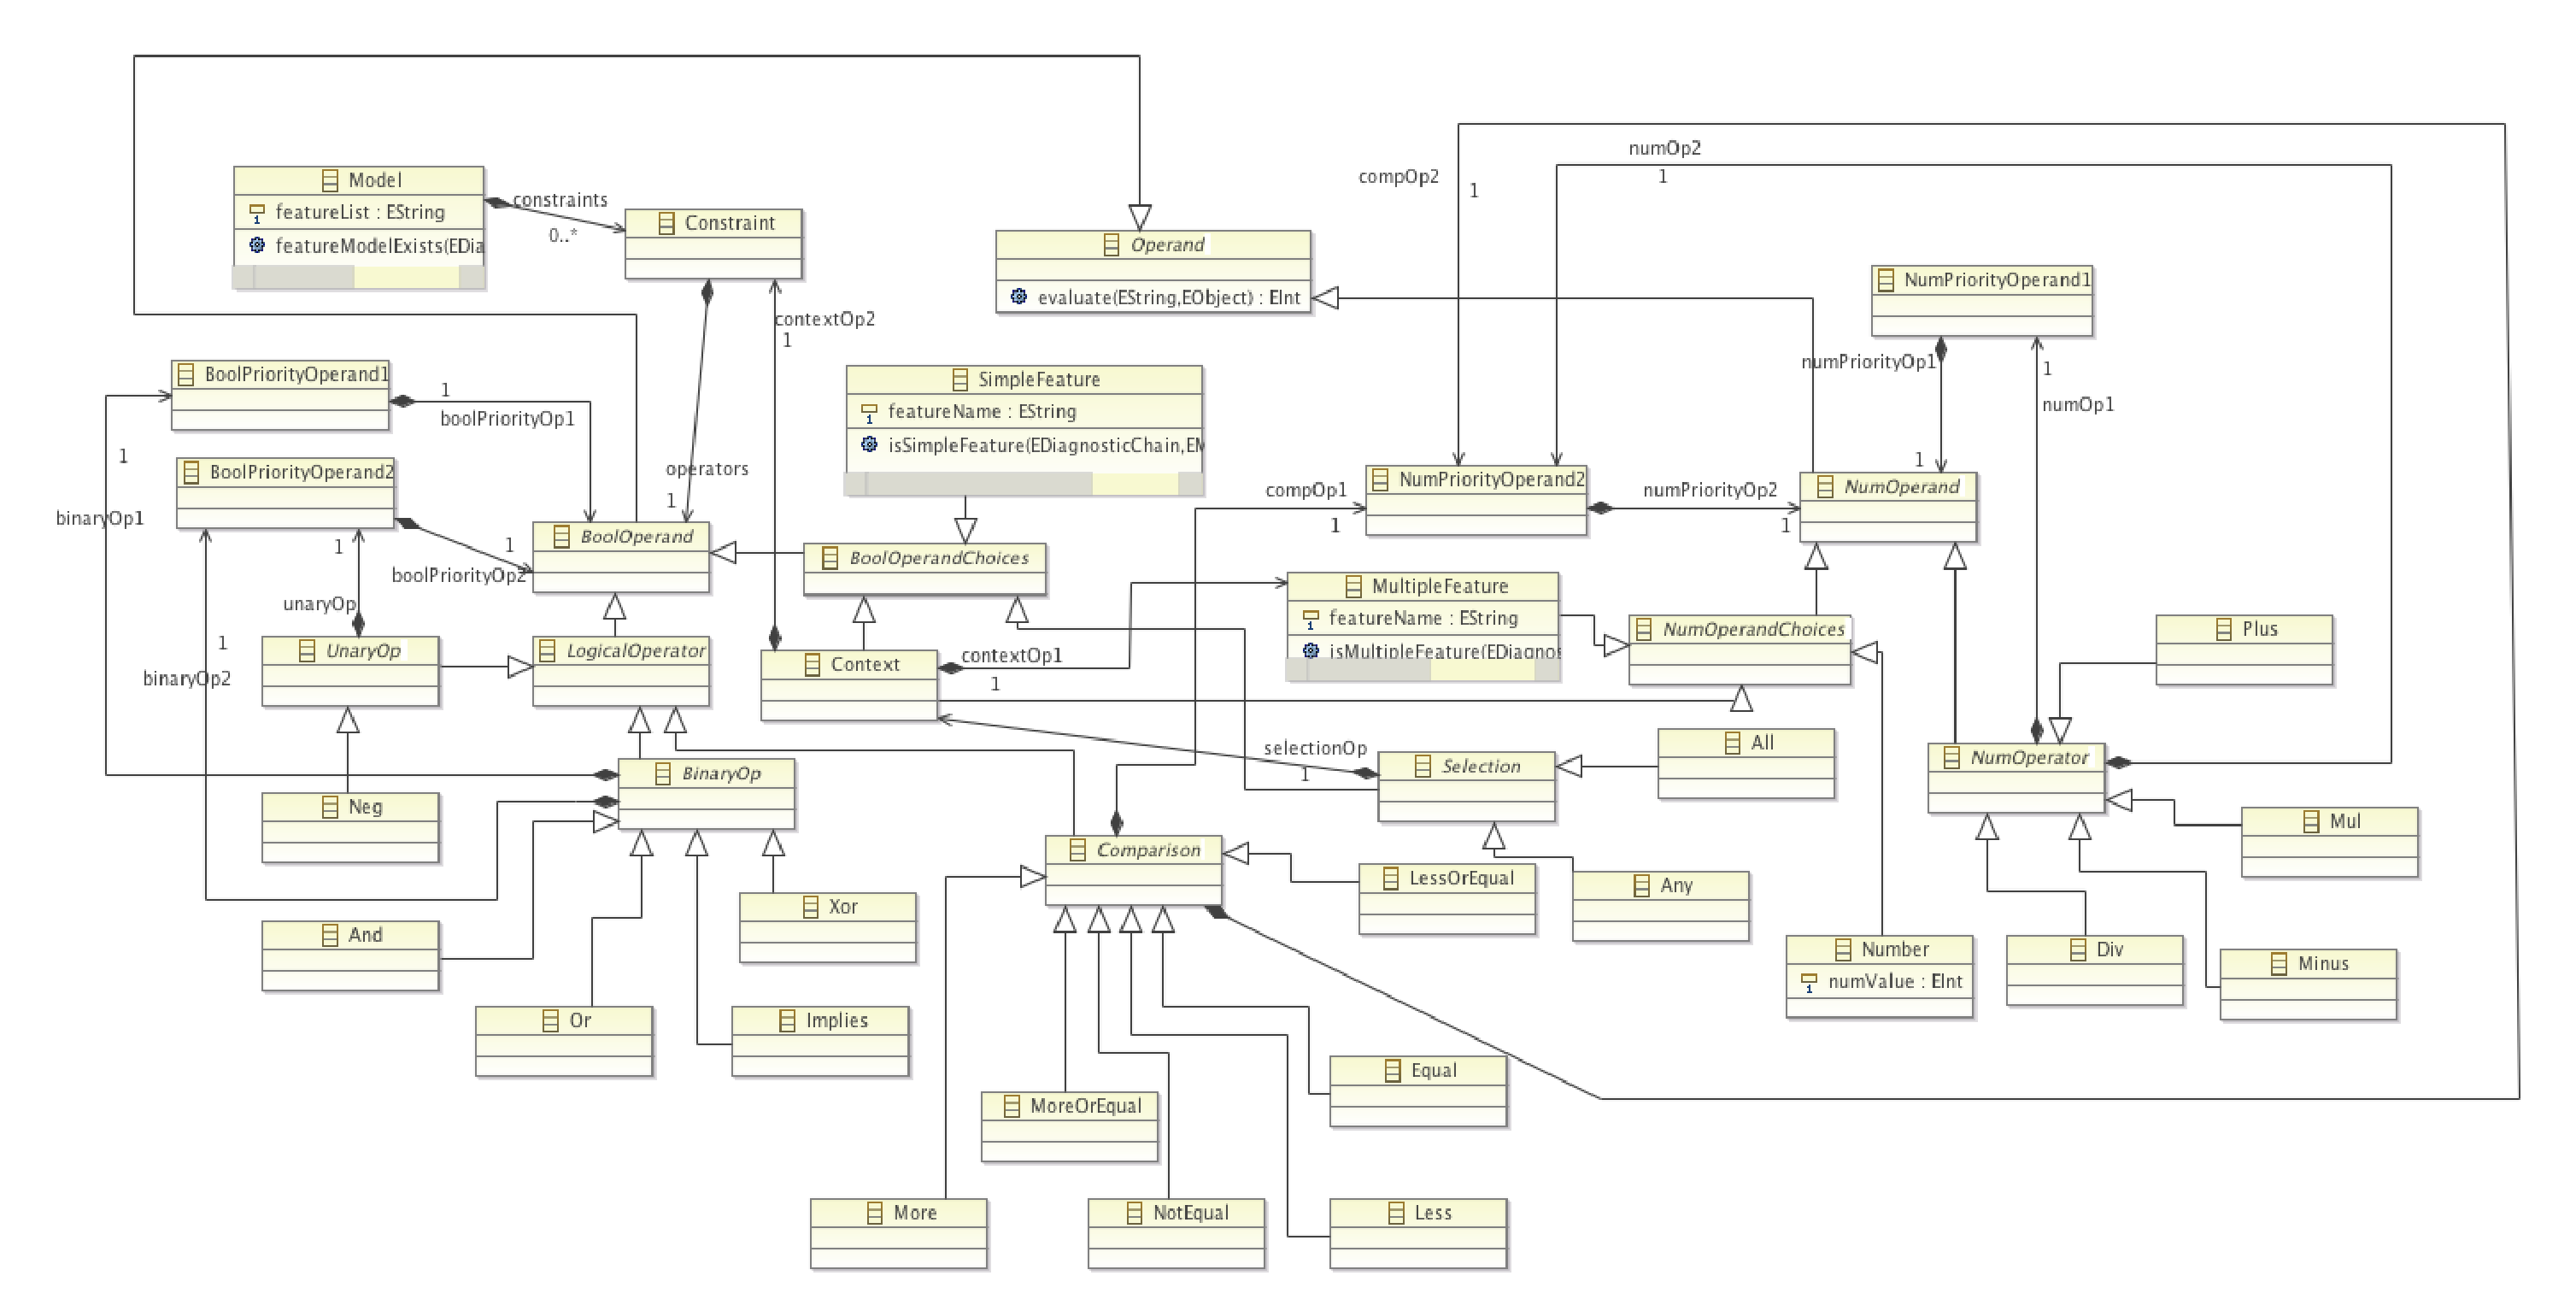
\includegraphics[scale=0.38, angle=90]{metamodelo/metamodelo.eps}}
    \caption{Metamodelo para el lenguaje HCL}
    \label{figmetameta}
\end{figure}

La clase \emph{Model} es la que sirve de punto de entrada y contender para el resto de las clases de nuestro metamodelo. 

C�mo se ha comentado anteriormente, debemos vincular un conjunto de restricciones con el �rbol de caracter�sticas al cual deben aplicarse. Dicho �rbol de caracter�sticas debe haber sido previamente creado usando la herramienta \emph{Hydra}, de acuerdo con los objetivos generales del proyecto. Eso reduce mucho el n�mero de factores de los que hay preocuparse, vi�ndose reducidos en este punto a tener que almacenar �nicamente la localizaci�n del fichero que contiene dicho �rbol de caracter�stica, con objeto de poder cargarlo cuando se necesite. La ruta de dicho fichero se almacena en el atributo \emph{featureList} de la clase \emph{Model}.

Un modelo de restricciones permite especificar un n�mero indeterminado de restricciones, representadas por la clase \emph{Constraint}. Por tanto, la clase \emph{Model} contendr� 0 o m�s restricciones (en principio se permiten definir ficheros sin restricciones, que se entiende se refinar�n postriormente). 

Una restricci�n es una expresi�n booleana que se eval�a a vedadero o falso, y que contendr� un operador booleano, representando por la clase \emph{BoolOperand}, y varios operadores, representados por diversas clases. 

Un operador booleano puede ser tanto una \emph{SimpleFeature}, es decir, una caracter�stica no clonable, como una operaci�n cuya evaluaci�n de como resultado un valor booleano. Estas operaciones pueden ser l�gicas (\emph{and}, \emph{or}, \emph{implies}, \emph{xor} y \emph{not}), de comparaci�n ($<$, $<=$, $>$, $>=$, =, !=), de selecci�n (\emph{all} y \emph{any}) o de contexto.

Por otro lado, una restricci�n tambi�n puede contener operadores num�ricos. Un operador num�rico puede ser una \emph{MultipleFeature}, es decir, una caracter�stica clonable, un n�mero, o una operaci�n cuya evaluaci�n de como resultado un valor num�rico. Estas operaciones son artim�ticas, es decir, $+$, $-$, $*$ y $/$. El operador m�s prioritario de una restricci�n siempre ha de ser booleano, pues en �ltima instancia esta tiene que poder ser evaluada a verdadero o falso.

Las operaciones l�gicas y num�ricas descritas est�n representadas en el metamodelo mediante las metaclases que llevan su nombre. Es decir, \emph{LessOrEqual} es la operaci�n $<=$, \emph{Plus} es la operaci�n $+$, y as� sucesivamente. Se puede apreciar que estas metaclases son las hojas de una estructura de herencias. Esta estructura permite no solo facilitar la comprensi�n del metamodelo, sino tambi�n servir de apoyo a \emph{EMFText} en el momento de construir la posterior gram�tica. 

Como ejemplo, vamos a seguir esta estructura a trav�s de una de las operaciones, \emph{Implies}. Esta metaclase hereda de \emph{BinaryOp}, que es la metaclase que representa las operaciones l�gicas con dos operandos. \emph{BinaryOp} a su vez hereda de \emph{LogicalOperator}, que representa las operaciones l�gicas. Por �ltimo, \emph{LogicalOperator} hereda de \emph{BoolOperand}, que representa los operadores booleanos. Un an�lisis an�logo se podr�a realizar con cualquiera de las operaciones implementadas.

Cabe tambi�n mencionar algunas metaclases como \emph{BoolPriorityOperand1} que parecen ajenas a esta estructura y cuya presencia puede resultar dudosa. Su inclusi�n se justifica por razones de funcionamiento de la herramienta \emph{EMFText}, que requiere un tratamiento especial a la hora de implementar prioridad entre las operaciones.

Los atributos de las metaclases sirven para almacenar informaci�n importante para el lenguaje, que posteriormente podr�a ser utilizada a nivel de validaci�n o ejecuci�n. De estos atributos ya se ha mencionado la utilidad de \emph{featureList}, dentro de la clase \emph{Model}. Adem�s de este, el atributo \emph{featureName} de las clases \emph{SimpleFeature} y \emph{MultipleFeature} sirve para almacenar el nombre de la caracter�stica a la que hagan alusi�n. Por �ltimo, el atributo \emph{numValue} de la clase \emph{Number} sirve para guardar el valor literal num�rico que haya sido introducido.

%\todo{sigue t� describiendo el metamodel o en este estilo, describiendo su estructura sin entrar en detalles ni ponerte demasiado barroco. Describes lo que hay, no el proceso de c�mo lo hiciste ni si te cost� m�s o menos, o te pareci� f�cil o dificil. No describas las asociaciones entre metaclases, eso es demasiado detalle}.

%%========================================================================================%%
%% NOTA(Pablo): Todo lo de abajo quedar� redundante con el nuevo texto, as� que mejor     %%
%%              eliminarlo                                                                %% 
%%========================================================================================%%

%%========================================================================================%%
%% INICIO DE PARTE POSIBLEMENTE REDUNDANTE                                                %%
%%========================================================================================%%

%El primer paso es definir toda la estructura necesaria para la implementaci�n de las operaciones, haciendo que cada una de ellas est� representada en nuestro metamodelo mediante una clase, pero sin preocuparnos todav�a por las relaciones entre ellas. La clase ra�z de toda esta estructura es Operand. Es una clase abstracta, es decir, en los modelos que luego instanciemos de este metamodelo no podr� haber ninguna instancia de Operand, s�lo de los hijos no abstractos que tenga. A medida que vayamos definiendo clases hijas  de Operand estaremos especificando cada vez con m�s exactitud a qu� tipo de operaci�n estamos haciendo referencia.
%
%En el segundo nivel de la estructura de implementaci�n de las operaciones hacemos una ramificaci�n seg�n el tipo del valor de retorno o de evaluaci�n de las posibilidades. Es decir, a la clase Operand le a�adiremos dos hijos: BoolOperand para operaciones que se eval�an a booleano y NumOperand para operaciones que se eval�an a num�rico. Estas clases tambi�n ser�n abstractas.
%
%El proceso de divisi�n a partir de aqu� es m�s o menos an�logo para todas las operaciones, as� que vamos a centrarnos �nicamente en la rama que da lugar a las operaciones binarias l�gicas, para comentar despu�s los casos y situaciones especiales. Una vez tenemos la clase BoolOperand, podemos especializarla un poco m�s a LogicalOperator, que a su vez se dividir� en operaciones unarias, binarias, o de comparaci�n. Todas ellas son clases abstractas. Por fin, la clase BinaryOp heredar� las clases de las operaciones propiamente dichas, en este caso And, Or, Implies y Xor. Estas ya podr�n ser instanciadas en las sintaxis concretas que creemos.
%
%Cabe hacer menci�n tambi�n a las clases SimpleFeature, MultipleFeature y Number, que representan a las caracter�sticas simples, m�ltiples y n�meros respectivamente. En cualquier �rbol resultante de parsear nuestro lenguaje, estas clases representar�n las hojas. En �ltima instancia todas las operaciones tendr�n como operandos caracter�sticas o n�meros. Podemos observar que SimpleFeature es un operando booleano (est� en la parte estructural de las operaciones booleanas) ya que su evaluaci�n ser� verdadero o falso, dependiendo si esa caracter�stica ha sido seleccionada en la configuraci�n correspondiente o no. MultipleFeature sin embargo se eval�a a n�mero entero. Su valor ser� el n�mero de apariciones de esa caracter�stica dentro de la configuraci�n correspondiente.
%
%Muchas de las clases que ahora se pueden contemplar en el metamodelo de la figura \ref{figmetameta} a�n no estaban presentes en esta etapa temprana del dise�o, y su inclusi�n fue necesaria a ra�z de la creaci�n de la gram�tica y los problemas que se observaron en ese punto. En particular, las terminadas en Choices y en PriorityOperand. Las operaciones All, Any y Context en este momento eran simples herencias de BoolOperand. El motivo de estas modificaciones ser� explicado en el cap�tulo siguiente.
%
%Para terminar este apartado, vamos a hablar de las relaciones entre las diferentes clases de nuestro metamodelo. En este punto del dise�o no eran las mismas que las de la figura \ref{figmetameta} por los motivos explicados anteriormente. Simplemente busc�bamos una forma de relacionar cada operaci�n con los tipos de sus operandos (que tambi�n pueden ser operaciones, como es l�gico). Las operaciones l�gicas binarias tendr�n dos operandos que tambi�n ser�n binarios. En este momento del dise�o binaryOp1 y binaryOp2 iban relacionados a BoolOperand, al igual que unaryOp. Del mismo modo, compOp1, compOp2, numOp1 y numOp2 (es decir, los operandos de operaciones de comparaci�n y num�ricas respectivamente) estaban relacionados con la clase NumOperand.
%
%La relaci�n de toda estructura de operaciones con los dos elementos anteriores, Model y Constraint, se realiza entre Constraint y BoolOperand. Toda restricci�n en �ltima ha de ser evaluada a verdadero o falso, es por eso que la relaci�n no va con Operand, como podr�a pensarse en primera instancia. De este modo estamos forzando que la operaci�n con menos profundidad del �rbol parseado de nuestra restricci�n sea booleana, y que por lo tanto el resultado final de validar la restricci�n sea un dato booleano.
%
%Quiz�s a alguien le pueda sorprender el hecho de que la relaci�n ''operators'' entre Constrain y BoolOperand sea 1..1 y no 1..*. El motivo es que como los operadores de esa primera operaci�n booleana que estamos forzando pueden ser a su vez operaciones, la complejidad en la restricci�n que podemos definir se propaga por ah� en lugar de por la relaci�n creada.

%%========================================================================================%%
%% FIN DE PARTE POSIBLEMENTE REDUNDANTE                                                   %%
%%========================================================================================%%

Como se coment� en la Secci�n~\ref{sec:intr:sle}, no todas las restricciones que debe satisfacer un lenguaje pueden especificarse mediante la notaci�n propia de un languaje de metamodelado. Para especificar dichas restricciones, se utilizan lenguajes complementarios al lenguaje propio de metamodelado. La siguiente secci�n explica como se definen dichas restricciones para nuestro lenguaje utilizando el EMF Validation Framework.




\section{Pruebas del metamodelo}
\label{sec:meta:pruebas}
%%==================================================================%%
%% Author : Tejedo Gonz�lez, Daniel                                 %%
%%          S�nchez Barreiro, Pablo                                 %%
%% Version: 1.0, 25/11/2012                                         %%
%% Version: 1.0, 06/02/2013                                         %%
%%                                                                  %%
%% Memoria del Proyecto Fin de Carrera                              %%
%% Sintaxis abstracta,  pruebas                                     %%
%%==================================================================%%

Una vez creado nuestro metamodelo, deb�amos probar que dicho metamodelo era correcto. Es decir, que permit�a especificar todas las restricciones que dese�bamos crear, a la vez que, por construcci�n, imped�a la especificaci�n de restricciones que deb�an ser consideradas como sint�cticamente incorrectas.

Para ello realizamos una serie de pruebas consistentes en la creaci�n de varias instancias del metamodelo y observar el �rbol de sintaxis abstracta generado, comprobando si �ste se correspond�a con el esperado.

\begin{figure}[t]
    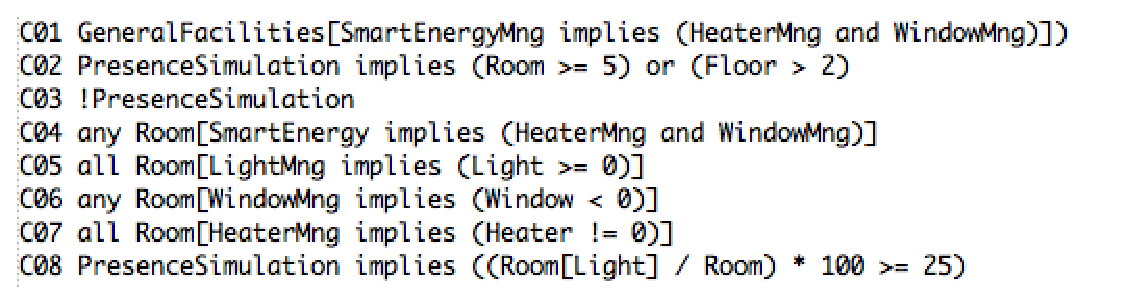
\includegraphics[scale=0.6]{metamodelo/instpruebas.eps}
    \caption{Conjunto de instrucciones que puso a prueba el funcionamiento del metamodelo}
    \label{figmetains}
\end{figure}

Las instrucciones que fueron puestas a prueba fueron las que se ven en la Figura~\ref{figmetains}. Este conjunto de instrucciones servir�n como pruebas tambi�n en momentos m�s avanzados del desarrollo. Dicho conjunto de pruebas fue dise�ado para recoger de la forma m�s exhaustiva posible todas las combinaciones de metaclases posibles.

